\section{Base Teórica}

La planificación es un componente esencial de cualquier sistema operativo, encargado de asignar tiempo de procesamiento a los diferentes hilos y procesos en ejecución. En este capítulo, nos sumergiremos en la comprensión de la planificación a corto plazo, con especial atención en el contexto del sistema operativo FreeBSD y su planificador 4BSD. Como ya se detalló previamente en el capítulo 1, este trabajo se basa y extiende directamente desde investigaciones previas\cite{bib1}, donde se introdujo el concepto de Redes de Petri, para el modelado de procesos.\par

Exploraremos los conceptos fundamentales de procesos e hilos, detallando su estructura, estados y dinámicas de ejecución. Además, nos adentraremos en el funcionamiento interno del planificador, desglosando las operaciones esenciales como el cambio de contexto, el encolado de procesos, la selección de procesador y la remoción de hilos de la cola. Estos aspectos son esenciales para comprender cómo el planificador 4BSD toma decisiones en tiempo real sobre la ejecución de procesos y la administración de recursos.\par

Al profundizar en esta base teórica, no solo sentaremos las bases para entender el funcionamiento del planificador de FreeBSD, sino que también estableceremos una sólida conexión con los avances y las decisiones tomadas en trabajos anteriores. Esto nos permitirá visualizar el progreso continuo y las oportunidades de mejora que surgieron a partir de esos primeros cambios implementados en el sistema operativo.\par

\subsection{Procesos e hilos}

En sistemas operativos, los procesos son entidades aisladas que representan la ejecución de una tarea o aplicación en particular. Cada proceso cuenta con su propio espacio de direcciones, que es un área reservada de memoria virtual donde se aloja el código del programa, las variables y los recursos necesarios para su ejecución. Además, disponen de acceso a los recursos del kernel a través de llamadas a sistemas.\par

Dentro de cada proceso, puede haber uno o varios hilos de ejecución. Estos hilos son unidades de ejecución independientes que comparten los recursos del proceso padre. Cada hilo se asocia con un procesador virtual, que tiene su propio contexto y un stack de ejecución alojado en el espacio de direcciones del proceso.\par

El kernel del sistema operativo crea la ilusión de ejecución concurrente de múltiples procesos, distribuyendo los recursos del sistema entre los procesadores listos para ejecutar tareas.\par

\subsubsection{Estructura de los procesos}
Cada proceso en el sistema recibe un identificador único llamado \textit{identificador de proceso} (PID). Los PID son el mecanismo común utilizado por las aplicaciones y el kernel para hacer referencia a los procesos. Existen dos identificadores que son de especial importancia para cada proceso: el PID del proceso en sí, y el PID del proceso padre.

La estructura simplificada de un proceso se puede observar en la Figura \ref{fig:process-state}. Esta estructura tiene como objetivo facilitar la gestión de múltiples hilos que comparten un espacio de direcciones y otros recursos dentro del proceso. Algunas de las categorías que componen esta estructura son las siguientes:

\begin{itemize}
    \item Identificación del grupo de procesos: el grupo de procesos y la sesión a la que pertenece el mismo son elementos importantes para la gestión y el control de los procesos en el sistema.
    \item Credenciales de usuario: los identificadores de usuario y grupo determinan los permisos de acceso a los recursos del sistema.
    \item Gestión de memoria: esta parte de la estructura es crucial para asignar y gestionar el espacio de direcciones virtuales del proceso, así como para administrar otros aspectos relacionados con la memoria.
    \item Descriptores de archivos: una matriz de punteros que indica los archivos abiertos por el proceso e información relevante de los mismos.
    \item Vector de llamadas al sistema: estructura de datos que mapea las llamadas al sistema con las funciones correspondientes en el kernel del sistema operativo.
    \item Contabilidad de recursos: estructura que describe la utilización de los recursos del sistema por parte del proceso.
    \item Estadísticas: estadísticas del proceso sobre su ejecución, temporizadores y profiling.
    \item Acciones de señal: la acción a tomar cuando se envía una señal a un proceso.
    \item Estructura de hilo: el contenido de la estructura de hilos del proceso.
\end{itemize}

\begin{figure}[H]
    \centering
    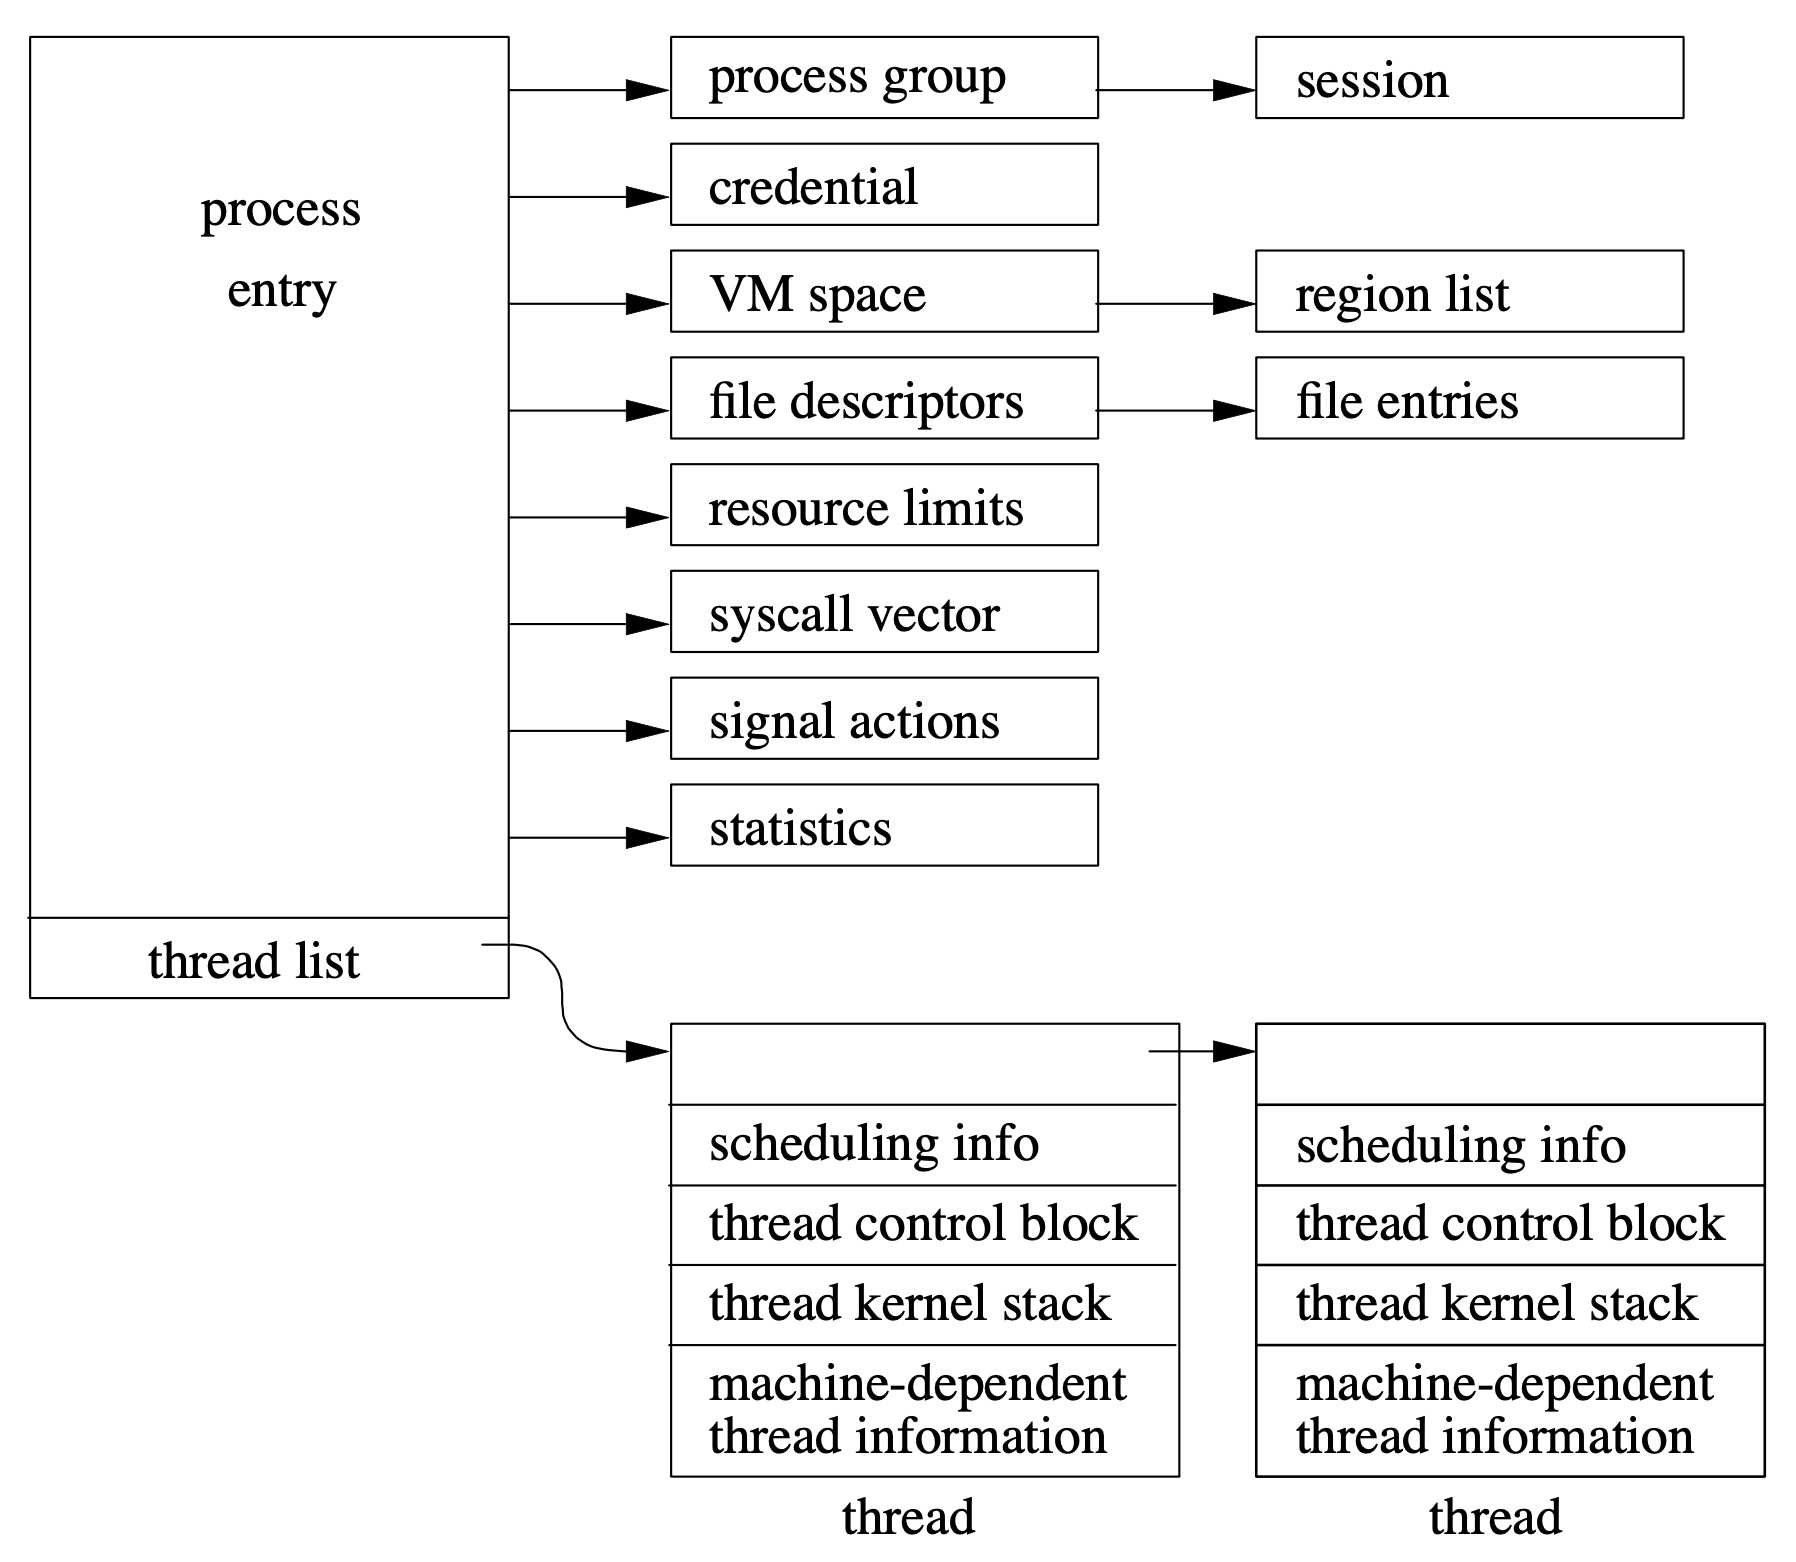
\includegraphics[width=0.5\textwidth]{./images/processStructure.png}
    \caption{Estructura simplificada de un proceso.}
    \label{fig:process-state}
\end{figure}

Cada proceso cuenta con los punteros \textit{p\_pptr}, \textit{p\_children} y \textit{p\_sibling}, utilizados para establecer la relación entre procesos. Cuando se crea un proceso hijo, se agrega a la lista \textit{p\_children} de su padre. El proceso hijo también mantiene un enlace a su padre mediante su puntero \textit{p\_pptr}. Si un proceso tiene más de un hijo activo al mismo tiempo, los hijos están asociados entre sí a través de las entradas de la lista \textit{p\_sibling}. La Figura \ref{fig:process-hierarchy} muestra un ejemplo de jerarquía de procesos.

\begin{figure}[H]
    \centering
    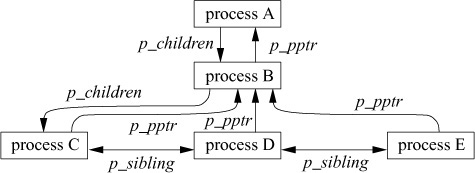
\includegraphics[width=0.5\textwidth]{./images/process-hierarchy.jpeg}
    \caption{Jerarquía de grupo de procesos.}
    \label{fig:process-hierarchy}
\end{figure}


\subsubsection{Estructura de los hilos}
Un hilo, en sistemas operativos modernos, constituye una unidad fundamental de ejecución dentro de un proceso. Se trata de una entidad independiente que representa una secuencia de instrucciones ejecutables dentro del contexto de un proceso. Cada hilo posee su propio contador de programa, registros de CPU y pila de ejecución, lo que le permite ejecutar código de manera concurrente dentro del mismo proceso. Aunque los hilos comparten recursos como el espacio de direcciones y otros recursos del proceso principal, también pueden comunicarse y cooperar entre sí para llevar a cabo tareas específicas de manera más eficiente.\par

En el caso de FreeBSD, el sistema adopta el modelo 1:1, donde cada hilo de usuario se corresponde con un hilo a nivel de kernel para mejorar la eficiencia de las aplicaciones.\par

La estructura de un hilo, que se muestra en la Figura \ref{fig:process-state}, contiene la información necesaria para ejecutarse en el kernel del sistema operativo:

\begin{itemize}
    \item Información para la planificación: se refiere a la prioridad del hilo en modo kernel y en modo usuario, la cantidad de tiempo que ha pasado suspendido y el uso reciente de la CPU. Además, se indica el estado de ejecución del hilo, banderas de estado adicionales; y si el hilo se encuentra suspendido, información sobre el canal y evento por el cual espera.
    \item TSB (thread state block): estado de ejecución del hilo en modo usuario y modo kernel. La estructura incluye registros de propósito general, punteros de pila, contador de programa, registros de gestión de memoria, entre otros.
    \item Pila del kernel: pila para usar al ejecutar en el kernel. Las pilas del kernel deben mantenerse pequeñas para evitar desperdiciar memoria física.
    \item Estado de la máquina (\textit{machine-dependent state}): se refiere a la información del hilo en relación a detalles que son específicos de la arquitectura de la CPU (registros de estado de punto flotante, información de interrupciones, información de registros de segmento de memoria, etc.).
\end{itemize}

\subsubsection{Estados de los procesos e hilos}

La estructura de un proceso en FreeBSD incluye un campo que indica su estado actual. Los estados de un proceso son fundamentales para entender su comportamiento en el sistema y están estrechamente relacionados con el funcionamiento del planificador 4BSD. Cuando se crea un proceso utilizando la llamada al sistema \textit{fork}, inicialmente se marca como nuevo (NEW). Este estado indica que el proceso está en su fase de creación y aún no ha recibido suficientes recursos para comenzar la ejecución.

Una vez que se asignan los recursos necesarios, el estado del proceso se cambia a NORMAL. En este estado, los hilos del proceso pueden encontrarse en diferentes subestados: ejecutable (RUNNABLE) cuando están listos para ejecutarse o actualmente en ejecución, durmiendo (SLEEPING) cuando están esperando un evento, o detenidos (STOPPED) cuando han sido pausados por una señal o por el proceso padre. El estado NORMAL persiste hasta que el proceso completa su tarea.

Cuando un proceso ha finalizado su ejecución, entra en el estado ZOMBIE. En este estado, el proceso ha liberado sus recursos pero aún no ha notificado formalmente su terminación al proceso padre. Es responsabilidad del sistema operativo limpiar los procesos en estado ZOMBIE y comunicar al proceso padre que el hijo ha finalizado.

La relación entre estos estados y el planificador 4BSD es crucial para comprender cómo se gestionan los recursos del sistema y cómo se asigna el tiempo de CPU a los procesos en FreeBSD.

En la tabla \ref{tabla:estados-proceso}, se proporciona una descripción concisa de cada estado del proceso y su significado en el contexto del sistema operativo.

\begin{table}[H]
    \centering
    \begin{tabular}{|c|p{0.8\textwidth}|}
        \hline
        \textbf{Estado} & \textbf{Características}                                                                             \\
        \hline
        NEW             & En fase de creación, aún sin recursos asignados                                                      \\
        \hline
        NORMAL          & Ejecución activa, sus hilos alternaran entre \textit{RUNNABLE}, \textit{SLEEPING} o \textit{STOPPED} \\
        \hline
        ZOMBIE          & En fase de finalización                                                                              \\
        \hline
    \end{tabular}
    \caption{Descripción de los estados del proceso en FreeBSD}
    \label{tabla:estados-proceso}
\end{table}

En FreeBSD, el sistema organiza las estructuras de procesos en dos listas principales: \textit{zombproc} y \textit{allproc}. Los procesos en estado ZOMBIE se encuentran en la lista \textit{zombproc}, mientras que los procesos activos están en la lista \textit{allproc}. Esta distinción permite optimizar las operaciones del sistema, como la llamada al sistema \textit{wait} que busca procesos terminados, así como las operaciones del planificador que identifican procesos listos para ejecutarse.

Los hilos de un proceso, por su lado, excluyendo los que están en ejecución, se distribuyen en tres colas principales: \textit{run\_queue}, \textit{sleep\_queue} y \textit{turnstile\_queue}. Los hilos listos para ejecutarse se ubican en la \textit{run\_queue}, mientras que aquellos que están bloqueados esperando eventos se encuentran en la \textit{sleep\_queue} o en la \textit{turnstile\_queue}. Es importante destacar que las colas \textit{run\_queue} están organizadas según la prioridad de planificación de hilos establecida por el planificador 4BSD. La diferencia entre la \textit{turnstile\_queue} y la \textit{sleep\_queue}, radica en que esta última se utiliza para hilos bloqueados con locks de tipo \textit{sleepable}, mientras que la \textit{turnstile\_queue} alberga hilos bloqueados con locks de tipo \textit{non-sleepable}.

\subsubsection{Prioridad de los hilos}

Las prioridades de los hilos son un componente importante para la planificación. Estas prioridades, que van desde 0 hasta 255 (donde 0 denota la prioridad más alta), determinarán el orden en que se ejecutarán los hilos. En la Tabla \ref{tabla:prio-hilos}, se describen los diferentes rangos de prioridades.

Las prioridades en el rango de 0 a 47 son asignadas de forma predeterminada por el sistema y se destinan a las tareas de interrupción.\par

Las prioridades de los hilos en tiempo real se encuentran en el intervalo de 48 a 79 y deben ser configuradas previamente por las aplicaciones mediante la llamada al sistema \textit{rtprio}. A continuación, se encuentran los hilos con prioridades en el rango de 80 a 119, conocidos como hilos del kernel superior (top-half kernel threads). Estos hilos se encargan de gestionar operaciones críticas del kernel que afectan a todo el sistema.\par

Los hilos con prioridades entre 120 y 223 pertenecen a la clase de hilos de tiempo compartido. Están destinados a ejecutar tareas de usuario convencionales y sus prioridades son ajustadas de manera automática por el kernel en función del uso de la CPU.\par

Cuando no hay tareas activas que requieran el uso de la CPU, los hilos de la clase \"IDLE\" pueden ejecutarse. Estos hilos tienen la finalidad de mantener el sistema en un estado inactivo, consumiendo recursos mínimos y estando listos para responder a tareas prioritarias.\par

\begin{table}[H]
    \centering
    \begin{tabular}{|c|c|c|}
        \hline
        \textbf{Rango} & \textbf{Clase} & \textbf{Tipo de hilo}          \\
        \hline
        0 - 47         & ITHD           & Bottom-half kernel (interrupt) \\
        \hline
        48 -79         & REALTIME       & Real-time user                 \\
        \hline
        80 - 119       & KERN           & Top-half kernel                \\
        \hline
        120 - 223      & TIMESHARE      & Time-sharing user              \\
        \hline
        224 - 255      & IDLE           & Idle user                      \\
        \hline
    \end{tabular}
    \caption{Clases de hilos por rango de prioridad.}
    \label{tabla:prio-hilos}
\end{table}


\subsection{Planificación}

La planificación en sistemas operativos, implica decidir el orden y la duración de la ejecución de procesos e hilos del sistema. En este sentido, es el componente clave para optimizar el uso de recursos y el tiempo de ejecución de los programas.\par

FreeBSD cuenta con el planificador 4BSD, un planificador de tiempo compartido (\textit{timeshare scheduler}) que asigna dinamicamente la prioridad de los procesos. El cálculo se realiza en función de varios parámetros de comportamiento previo de dicho proceso, como la cantidad de tiempo de CPU utilizado, la cantidad de recursos de memoria que posee o requiere para su ejecución, entre otros.\par

La política de planificación asigna inicialmente una prioridad de ejecución alta a cada hilo y permite que ese hilo se ejecute durante un intervalo de tiempo fijo, o \textit{time slice}. A los hilos que se ejecutan durante la duración de su \textit{time slice} se les decrementa la prioridad; mientras que los hilos que ceden la CPU (generalmente debido a operaciones de entrada/salida) pueden mantener su prioridad. Por otro lado, los hilos inactivos incrementan su prioridad.\par

Esta forma de planificación beneficia especialmente a los programas interactivos. Los procesos que demandan una gran cantidad de tiempo de CPU ven reducida rápidamente su prioridad, mientras que los procesos interactivos que permanecen mayormente inactivos conservan una prioridad elevada. Esto permite que, cuando estén listos para ejecutarse, puedan desplazar a los procesos de baja prioridad que llevan ejecutándose durante un largo período de tiempo. Por ejemplo, supongamos que un editor de texto realiza una búsqueda dentro de un documento, lo que conlleva un aumento temporal en el uso de recursos computacionales. Durante este período, la prioridad del editor puede verse momentáneamente reducida para dar prioridad a otros procesos más urgentes. Sin embargo, una vez completada la búsqueda y sin actividad adicional del usuario, el editor recuperará su prioridad en la cola de planificación del sistema operativo.\par

Algunas tareas requieren un control más preciso sobre el proceso, como el caso de la planificación de tiempo real. FreeBSD también implementa esta funcionalidad mediante una cola separada para los hilos en cuestión, los cuales no se ven interrumpidos por otros hilos a menos que tengan igual o mayor prioridad. Además, el \textit{kernel} de FreeBSD cuenta con otra cola de hilos de mínima prioridad que se ejecutan únicamente cuando ningún hilo en las colas de mayor prioridad está en un estado de posible ejecución.\par

\subsubsection{\textit{Multilevel Feedback Queue Scheduling}}

El planificador 4BSD, utiliza un algoritmo de planificación basado en colas de retroalimentación multinivel \textit{Multilevel Feedback Queue}. Todos los hilos en estado \textit{RUNNABLE} reciben una prioridad que determina en qué cola de ejecución se colocan. Al seleccionar un nuevo hilo para ejecutar, el sistema escanea las colas de ejecución de mayor a menor prioridad y elige aquel que se encuentra en la primera cola no vacía. Si varios hilos residen en una cola, el sistema los ejecuta en orden circular (\textit{Round Robin}); es decir, en el orden en que se encuentran en la cola, con igual cantidad de tiempo permitido.\par

Si un hilo se bloquea, no se vuelve a colocar en la cola de ejecución (\textit{run\_queue}); en su lugar, se coloca en una \textit{turnstile\_queue} o en una \textit{sleep\_queue}. Cuando el hilo agota el \textit{time slice}, se coloca al final de la cola de la que provino y se selecciona el hilo que se encuentra al comienzo de la misma para ejecutarse.\par

Cuanto más corto sea el \textit{time slice}, mejor será la respuesta interactiva. Sin embargo, cuanto más largos sean los cuántums de tiempo, mayor será el rendimiento del sistema, ya que habrá menos sobrecarga debida a los cambios de contexto y se limpiarán menos a menudo las cachés del procesador. El \textit{time slice} utilizado por 4BSD es de 0.1 segundo. Este valor se encontró empíricamente como el cuántum más largo que podía usarse sin pérdida de la respuesta deseada para trabajos interactivos como los editores.\par

\subsubsection{Colas de ejecución de hilos y Cambios de Contexto}

El \textit{kernel} cuenta con un conjunto único de colas de ejecución para manejar todas las clases de hilos mencionadas anteriormente en la sección "Prioridad de los hilos". La cantidad de colas utilizadas para mantener la colección de hilos \textit{RUNNABLE} impacta en el costo de su gestión. Mantener una sola cola ordenada simplifica la operación de búsqueda y selección del próximo hilo listo, pero otras operaciones se vuelven más costosas. Por otro lado, si se utilizara una cola por cada nivel de prioridad, la selección del próximo hilo listo sería demasiado costosa, dado que habría que buscar entre 256 de ellas. FreeBSD emplea 64 colas de ejecución para los hilos listos, de modo que para ubicar un hilo en una cola, se divide la prioridad del mismo por 4, y el resultado indica la cola donde debería ser ubicado. Con el fin de optimizar el tiempo, los hilos en cada cola no son reordenados según sus prioridades.\par

Las colas de ejecución contienen todos los hilos listos en la memoria principal, excepto el hilo que se está ejecutando actualmente. La Figura \ref{fig:queueing-structure} muestra cómo se organiza cada cola como una lista doblemente enlazada de estructuras de hilo. La cabecera de cada cola de ejecución se mantiene en un arreglo. Asociado con este arreglo existe un vector de bits que se utiliza para identificar las colas de ejecución no vacías.\par

\begin{figure}[H]
    \centering
    \vspace*{0.2in}
    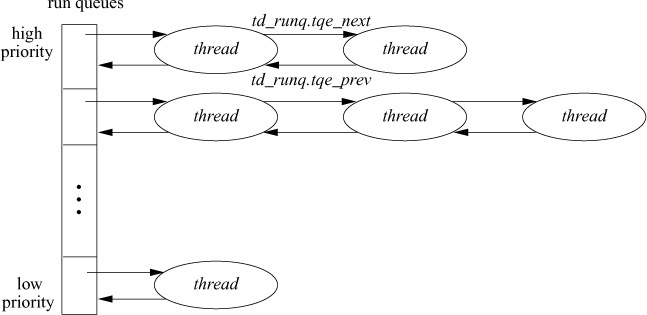
\includegraphics[width=0.8\textwidth]{./images/queueing-structure.jpg}
    \caption{Estructura de colas para hilos \textit{RUNNABLE}}
    \label{fig:queueing-structure}
\end{figure}

El código de cambio de contexto se divide en dos partes: una parte independiente de la máquina, que reside en \textit{mi\_switch()}, y otra parte dependiente de la máquina, que reside en \textit{cpu\_switch()}.\par

Los \textbf{cambios de contexto voluntarios}, es decir, cuando un hilo decide ceder la CPU de forma deliberada, ocurren cuando dicho hilo llama a la rutina \textit{sleep()}, colocándolo en una cola de espera e invocando \textit{mi\_switch()} para programar el siguiente hilo a ejecutar.\par

La rutina \textit{mi\_switch()} no puede ser llamada desde el código que se ejecuta a nivel de interrupción, ya que debe ser invocada dentro del contexto del hilo en ejecución. Por ello, para \textbf{cambios de contexto involuntarios}, se activa la bandera TDF\_NEEDRESCHED del hilo en ejecución y luego se envía una trampa de sistema asíncrona (AST). Una AST es una trampa que se le entrega al hilo que se estaba ejecutando previo a una interrupción, para que en lugar de reanudar su ejecución (al volver de la interrupción), se llame a la rutina \textit{mi\_switch()}.\par

\subsubsection{Planificador 4BSD para sistemas multiprocesador}

El planificador 4BSD en FreeBSD está diseñado para gestionar la carga de trabajo en sistemas multiprocesador mediante un enfoque que equilibra la carga de los procesadores. Para lograr esto, el planificador emplea tanto las colas de ejecución específicas de cada CPU como una cola de ejecución global. Tanto la cola global como las específicas de cada CPU están estructuradas como colas de múltiples niveles con realimentación (Multilevel Feedback Queue), lo que permite priorizar y gestionar los hilos de manera eficiente según su comportamiento y necesidades de tiempo de CPU.

La cola de ejecución global contiene hilos que pueden ser ejecutados por cualquier CPU del sistema. Sirve como un \textit{pool} central de hilos listos para ejecutarse, permitiendo una distribución flexible de la carga de trabajo. Cuando una CPU queda inactiva, revisa tanto su propia cola de ejecución como la cola de ejecución global, seleccionando el hilo con mayor prioridad para ejecutarlo. En los casos en donde la cola de ejecución propia está vacía, la CPU tomará un hilo de la cola global, garantizando que todas las CPUs tengan trabajo disponible si hay suficientes hilos listos para ejecutarse.

Por otro lado, cada CPU en el sistema tiene su propia cola de ejecución. Estas colas contienen hilos que están designados para ejecutarse en CPUs específicas. Para optimizar el rendimiento, el planificador 4BSD considera varias restricciones y preferencias de afinidad cuando decide dónde colocar un hilo cuando termina su \textit{time slice} o debe abandonar por otras razones.

Algunos hilos pueden estar vinculados a un conjunto específico de CPUs debido a consideraciones de rendimiento. El planificador 4BSD respeta esta afinidad al determinar en qué CPU encolar el hilo mediante un mecanismo de iteración sobre las CPUs asignadas al hilo, excluyendo aquellas para las que no existe afinidad. Luego, selecciona la CPU cuya cola tenga la menor cantidad de hilos listos para ejecutarse.\par

La función de \textit{bounding}, por otro lado, implica restringir un hilo a un procesador específico. Por ejemplo, al ejecutar el método \textit{kern\_reboot} en FreeBSD, encargado de preparar el sistema para un reinicio, apagado o parada, es necesario vincular primero dicho hilo al procesador 0. Esto garantiza que el código se ejecute en la CPU0, una práctica crucial en sistemas que solo permiten la ejecución de instrucciones en dicha CPU.\par

Por último, los hilos pueden ser \textit{pinned} o anclados a una CPU particular. Cuando un hilo está anclado, el planificador se asegura de encolarlo siempre en el último procesador en el que se ejecutó. En el contexto del kernel de FreeBSD, esto se realiza para mantener la coherencia de caché o para garantizar la eficiencia de la ejecución de tareas críticas evitando la migración del hilo entre CPUs durante su ejecución. El método que ancla un hilo, es el que finalmente libera al hilo de esta restricción.\par

\subsection{Conceptos del proyecto integrador previo}

En el contexto del proyecto integrador previo, se llevó a cabo un análisis detallado del comportamiento del \textit{scheduler} de un sistema operativo, con un enfoque específico en el proceso de asignación de tiempo de procesador. El objetivo fundamental fue identificar oportunidades de mejora en su funcionamiento, migrando de una visión estadística a un sistema más complejo implementado mediante Redes de Petri, en donde las decisiones de encolado de los hilos en una CPU se derivan de la información representada en el modelo, incluidos los estados globales y los de cada hilo.\par

En las secciones siguientes, se presentan los puntos clave abordados en este estudio, incluyendo la naturaleza de las modificaciones realizadas. Además, se resaltan los puntos de interés surgidos durante este análisis, los cuales orientarán el desarrollo de los distintos módulos destinados a ampliar las funcionalidades de planificación como la gestión del encendido y apagado de procesadores, así como la monopolización de los mismos por parte de los hilos.\par

\subsubsection{Elección del planificador}

La planificación a corto plazo en FreeBSD ha experimentado una evolución constante desde sus primeras versiones basadas en el sistema operativo 4.4BSD\cite{bib3}. A lo largo de su historia, FreeBSD ha confiado en dos planificadores para gestionar la asignación de recursos del sistema, siendo el planificador 4BSD uno de los más notables. Este planificador, inicialmente diseñado para sistemas monoprocesador, ha sido adaptado y optimizado para entornos multiprocesador, convirtiéndose en un componente fundamental de la arquitectura del sistema operativo.\par

Aunque el planificador 4BSD es más simple en comparación con los más modernos, ha demostrado ser rápido y eficiente para satisfacer las necesidades de muchos usuarios. Sin embargo, con el objetivo de mejorar aún más el rendimiento y la capacidad de respuesta del sistema, se introdujo el planificador ULE en la versión 5.0 de FreeBSD. El ULE ofrece características avanzadas que lo hacen más adecuado para entornos con cargas de trabajo más complejas y exigentes.\par

A pesar de que el planificador ULE se ha convertido en el predeterminado en las versiones más recientes de FreeBSD (a partir de la versión 8.0), el planificador 4BSD sigue siendo una opción estable y confiable. La comunidad de FreeBSD continúa manteniendo y brindando soporte para el planificador 4BSD, asegurando su disponibilidad para aquellos que prefieren su simplicidad y eficiencia. Además, no hay planes inmediatos por parte del equipo de desarrollo de FreeBSD para dejar de darle soporte.\par

Nuestro proyecto se basa en el trabajo previo que se centró en el planificador 4BSD. Para obtener una comprensión más detallada y contextualizada de esta elección, se puede consultar las secciones de \textit{Alcance} (1.4) y  \textit{Diferencias entre el planificador ULE y el 4BSD} (2.3.3) del proyecto integrador previo\cite{bib1}. Aunque nuestro enfoque principal no radica en realizar cambios inmediatos en el sistema operativo ni en contribuir directamente a la comunidad de FreeBSD, continuamos con la fase de investigación e implementación centrada en este tipo de planificadores.\par


\subsubsection{Análisis de modificaciones realizadas}

Como se explicó previamente, la planificación en sistemas operativos consiste en decidir el orden y la duración de la ejecución de los distintos hilos del sistema. Tradicionalmente, los sistemas operativos han basado estas decisiones en estadísticas del comportamiento previo, utilizando datos históricos para optimizar el rendimiento.

Un aspecto importante de esta planificación ocurre cuando un hilo debe ceder la CPU a otro. En el contexto del planificador 4BSD, esto implica retirar un hilo de la cola de ejecución (RUNNABLE) y ponerlo en ejecución, mientras que el hilo que estaba en ejecución vuelve a encolarse. Aquí es donde se enfocó el trabajo anterior: en modelar el sistema de encolado y desencolado de hilos utilizando redes de Petri. Esta técnica permite representar de manera precisa y formal los estados y transiciones de los hilos, mejorando así la eficiencia y previsibilidad del planificador.

Las modificaciones realizadas en el código del planificador 4BSD se centraron en adaptar las funciones principales para que se ajusten al uso de redes de Petri. Estos cambios se llevaron a cabo en el archivo \textit{sched\_4bsd.c}, que contiene las funciones principales del planificador 4BSD.

Para comprender la naturaleza de los cambios realizados en el trabajo previo, detallaremos los resultados finales en términos de modelado de sistemas mediante redes de Petri.

\subsubsection{Modelado del hilo}

Uno de los modelos representados mediante redes de Petri es el de los estados de un hilo, como se muestra en la Figura \ref{fig:threadModel}.\par

\begin{figure}[h]
    \centering
    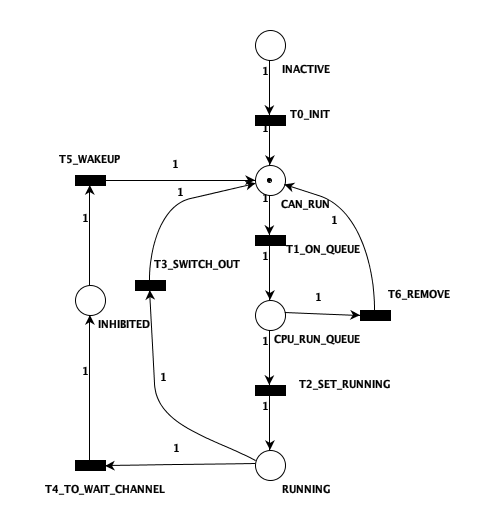
\includegraphics[width=0.45\textwidth]{images/Thread_Net.png}
    \caption{Modelo del hilo.}
    \label{fig:threadModel}
\end{figure}

Las plazas de la Red de Petri la Figura \ref{fig:threadModel} se corresponden a los estados posibles del hilo, siendo posible encontrarse en un solo estado a la vez. Las transiciones, por otro lado, representan los eventos que pueden llevar al hilo de un estado a otro. A continuación, se detallan las transiciones que se modelaron en la Red de Petri para el hilo:

\begin{itemize}
    \item \textbf{T0\_INIT}: Transición del estado INACTIVE a CAN\_RUN, que ocurre cuando el hilo se agrega al planificador. Esta tarea no corresponde al scheduler, por lo que inicialmente un hilo en el planificador se inicializa en el estado CAN\_RUN. Aunque esta transición no se dispara en la práctica, se incluyó en el modelo por razones representativas.
    \item \textbf{T1\_ON\_QUEUE}: El hilo se coloca en una cola local de una CPU específica o en la cola global, según la disponibilidad.
    \item \textbf{T2\_SET\_RUNNING}: El hilo se retira de la cola y comienza a ejecutar las instrucciones del programa asignado, ocupando así el procesador.
    \item \textbf{T3\_SWITCH\_OUT}: El planificador interrumpe el hilo y lo devuelve a su estado de CAN\_RUN, seleccionando otro hilo de mayor prioridad para ejecutar y realizando un cambio de contexto.
    \item \textbf{T4\_TO\_WAIT\_CHANNEL}: El hilo se bloquea debido a algún evento, semáforo o espera, y se coloca en una cola de espera hasta que se desbloquee.
    \item \textbf{T5\_WAKEUP}: El hilo se desbloquea y puede volver a encolarse. Este evento ocurre fuera del planificador, y el hilo espera cambiar de estado según corresponda.
    \item \textbf{T6\_REMOVE}: Se ejecuta cuando un hilo debe eliminarse de la cola en la que se encuentra.
\end{itemize}


\subsubsection{Modelado del planificador}

Por otro lado, se realizó el modelado de la red de Petri del planificador, o red de recursos, que se muestra en la Figura \ref{fig:schedulerModel}. En esta figura se detallan las plaza y transiciones de una sola CPU, siendo extensible a tantas CPUs como el sistema multiprocesador posea.

\begin{figure}[h]
    \centering
    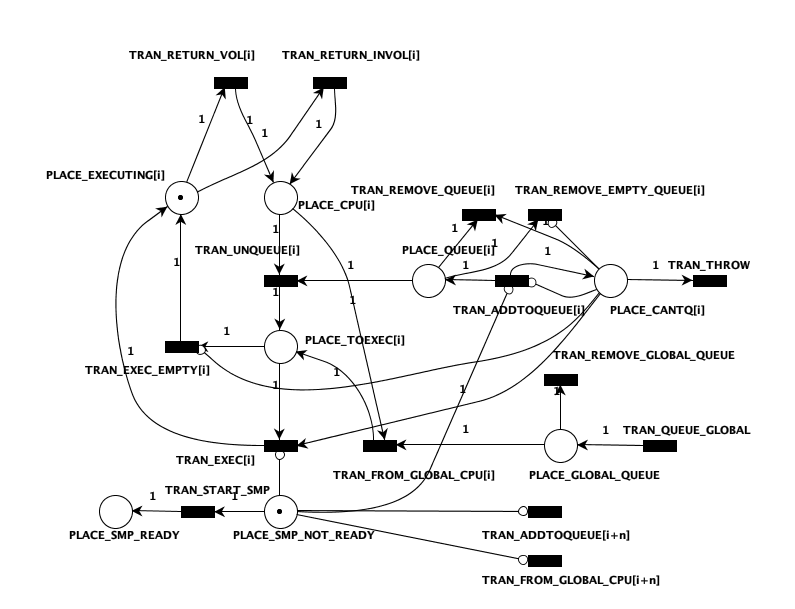
\includegraphics[width=0.8\textwidth]{images/Resource_1CPU.png}
    \caption{Modelo del planificador.}
    \label{fig:schedulerModel}
\end{figure}

Las plazas del planificador, podemos separarlas en las siguientes categorías:

\begin{itemize}
    \item \textbf{Plazas de la actividad del procesador}: Entre ellas encontramos las plazas PLACE\_CPU, PLACE\_TOEXEC y PLACE\_EXECUTING que representan el estado de ejecución de un hilo sobre el procesador en cuestión.
    \item \textbf{Plazas de colas del procesador}: PLACE\_QUEUE y PLACE\_CANTQ, que representan las colas del procesador en cuestión, con un sistema diseñado para soportar la penalización de procesadores.
    \item \textbf{Plazas globales o de sistema}: PLACE\_GLOBAL\_QUEUE, PLACE\_SMP\_READY y PLACE\_SMP\_NOT\_READY que representan las colas globales y el estado del sistema SMP en un determinado momento.
\end{itemize}

En cuanto a las transiciones de la red, podemos hacer la misma categorización:

\begin{itemize}
    \item \textbf{Transiciones de la actividad del procesador}:
        \begin{itemize}
            \item \textbf{TRAN\_UNQUEUE}: Esta transición elimina al hilo próximo a ejecutarse de la cola de la CPU, dejándolo listo para su ejecución.
            \item \textbf{TRAN\_EXEC}: El hilo pasa a ejecutarse, ocupando el recurso del procesador. Esta transición elimina el token de la plaza de habilitación, permitiendo que un nuevo hilo pueda ser encolado. Cabe destacar que esta transición está inhibida en modo monoprocesador ya que en este modo los hilos que se planifican, son buscados en la cola global.
            \item \textbf{TRAN\_EXEC\_EMPTY}: Similar a TRAN\_EXEC, esta transición permite la ejecución de hilos provenientes de la cola global.
            \item \textbf{TRAN\_RETURN\_VOL}: Representa la liberación del recurso del procesador para permitir la ejecución de otro hilo de la cola. Se dispara cuando un hilo no puede continuar su ejecución debido a la espera de un evento o recurso.
            \item \textbf{TRAN\_RETURN\_INVOL}: Al igual que TRAN\_RETURN\_VOL, esta transición se dispara cuando un hilo libera el procesador, pero en este caso, la interrupción se produce porque el hilo ha consumido su tiempo asignado de CPU o ha finalizado su tarea.
        \end{itemize}
    \item \textbf{Transiciones de colas del procesador}:
        \begin{itemize}
            \item \textbf{TRAN\_ADDTOQUEUE}: Un hilo se agrega a la cola de la CPU correspondiente. Esta transición está inhibida cuando el sistema está en modo monoprocesador (al inicio del sistema operativo) y cuando ya existe un hilo en la cola. Esta última decisión recae en un sistema de colas y de penalización de procesadores implementada en el trabajo integrador previo.
            \item \textbf{TRAN\_REMOVE\_QUEUE}: Expulsa un hilo de la cola y resta un token de habilitación de la CPU, desinhibiendo el encolado de otro hilo del sistema de penalización.
            \item \textbf{TRAN\_REMOVE\_EMPTY\_QUEUE}: Funciona igual que TRAN\_REMOVE\_QUEUE, pero se ejecuta cuando la plaza de habilitación no tiene ningún token.
            \item \textbf{TRAN\_THROW}: Esta transición se dispara automáticamente cuando todas las plazas de habilitación de las CPU tienen al menos un token. Su objetivo es habilitar las colas con la menor cantidad de hilos que estaban inhibidas, una vez que todas las colas se han nivelado.
        \end{itemize}
    \item \textbf{Transiciones globales o de sistema}:
        \begin{itemize}
            \item \textbf{TRAN\_FROM\_GLOBAL\_CPU}: Representa el desencolado de un hilo desde la cola global.
            \item \textbf{TRAN\_REMOVE\_GLOBAL\_QUEUE}: Expulsa un hilo de la cola global sin afectar la habilitación de la CPU.
            \item \textbf{TRAN\_START\_SMP}: Se dispara cuando el sistema cambia de monoprocesador a multiprocesador.
            \item \textbf{TRAN\_QUEUE\_GLOBAL}: Agrega un hilo a la cola global.
        \end{itemize}
    \end{itemize}


\subsubsection{Jerarquía de transiciones}
Para llevar a cabo la conexión entre las redes de los hilos y la red de recursos de las CPU se utiliza el concepto de redes jerárquicas. Es decir que al dispararse cierta transición en la red de recursos, también debe dispararse su transición correspondiente en la red del hilo.

Las jerarquías están definidas de la siguiente forma:

\begin{itemize}
    \item Transiciones TRAN\_ADDTOQUEUE y TRAN\_QUEUE\_GLOBAL de la red de recursos son jerárquicas a la transición T1\_ON\_QUEUE del hilo.
    \item Transiciones TRAN\_EXEC y TRAN\_EXEC\_EMPTY de la red de recursos son jerárquicas a la transición T2\_SET\_RUNNING del hilo.
    \item Transiciones TRAN\_REMOVE\_QUEUE, TRAN\_REMOVE\_EMPTY\_QUEUE y TRAN\_ REMOVE\_GLOBAL\_QUEUE de la red de recursos son jerárquicas a la transición T6\_ REMOVE del hilo.
    \item Transición TRAN\_RETURN\_INVOL de la red de recursos es jerárquica a la transición T3\_ SWITCH\_OUT del hilo.
    \item Transición TRAN\_RETURN\_VOL de la red de recursos es jerárquica a la transición T4\_TO \_WAIT\_CHANNEL del hilo.
\end{itemize}

\subsubsection{Marcado inicial}
La red de recursos se inicializará siempre con un token en la plaza que indica que el sistema se encuentra funcionando en modo monoprocesador. Además, se inicializan las plazas que representan a las CPU con un token, excepto la de la CPU0 ya que la misma, inicialmente se encuentra ejecutando el hilo inicial del sistema, por lo que esta última debe inicializarse con un token en la plaza de ejecución (PLACE\_EXECUTING\_0).



\subsubsection{Métodos de interes para nuestra tesis}

Las principales modificaciones realizadas en el planificador se encuentran en las siguientes funciones, donde se implementaron las transiciones correspondientes para asociar y ajustar el funcionamiento del planificador original, al modelo de la red de Petri:

\begin{itemize}
    \item Funciones de inicialización del planificador: Se añadieron funciones para inicializar la red de Petri, incluyendo el marcado inicial y la configuración de las transiciones y plazas en el modelo, representadas mediante variables.
    \item Encolado de hilos: En la función que gestiona el encolado de hilos, se ajustó la lógica para alinearse con la red de Petri, permitiendo que un hilo sea encolado en la cola global o en la de un procesador específico.
    \item Desencolado de hilos: En la función encargada de desencolar hilos, se integró el disparo de la transición correspondiente, permitiendo desencolar un hilo tanto de la cola global como de la cola de un procesador.
    \item Selección del hilo a ejecutar: En la función que elige el próximo hilo a ejecutar, se gestionan los hilos de la cola global, las colas de los procesadores y el hilo IDLETHREAD, ejecutado en casos de ausencia de otros hilos listos.
    \item Selección del Procesador: La función que selecciona el procesador adecuado para ejecutar un hilo fue completamente rediseñada para basarse en el estado de la red de Petri.
    \item Expulsión de Hilos: Función donde se gestiona la expulsión de hilos del planificador.
    \item Cambio de Contexto: Se añadieron las transiciones necesarias para tener en cuenta el cambio de contexto entre hilos debido a la preempción.
\end{itemize}
